\newpage
\section{Activity Based Costing}

\todo{CS: table refs are incorrect}

\subsection{Basic Concepts}

\subsubsection{Process Controlling}
Process controlling has both a strategic and an operational dimension [cf. e.g. \cite{book:ProzesseSchmelzer}, p. 229 ff.]. We concentrate on methods and techniques for planning, designing and coordinating the supply of information necessary to allow continuous operational process controlling with key figures as indicated in the closed-loop approach to performance management (see lower part of figure \ref{fig:Approach-Performance} in \ref{sec:BAMinSubjectOrientation}). As operational process controlling aims for post-execution analysis of business process instances it can be complemented by Business Activity Monitoring (BAM) which, based on event processing concepts, observes instances during execution and sets alerts or triggers actions in real-time or near real-time according to the particular situations identified (cf. \cite{book:processmonitoring}, \cite{article:BlueprintEventDriven}).
\\
The major question is how to measure process performance. A typical parameter for the evaluation of process effectivity is customer satisfaction while process time, quality and cost and adherence to schedules are suitable to assess efficiency (cf. e.g. \cite{book:ProzesseSchmelzer} p. 229 ff.). As these parameters have high significance for the competitive position they are crucial for process controlling. While the assessment of customer satisfaction and maturity levels of processes usually are matters of periodic monitoring activities there might be other, more technical parameters needed to be watched permanently, like the response time of application systems. Those aspects are especially relevant if processes are extensively supported by IT.
\\
Figure \ref{fig:OpProcessCont} gives a conceptual overview of a key figure-based operational process controlling, split into continuous and periodic or occasional controlling activities, like it could be set up successively for the S-BPM approach.
The integrated collection and analysis of common managerial data allows for a cohesive evaluation and control in terms of process controlling [cf. \cite{book:ProzesseSchmelzer} p. 248 ff., 1 p. 385 ff., 7 p. 158 ff.]. It feeds back results to take decisions and actions, fostering a steadily growth of experience regarding the interdependencies between cost, quality and time (organizational learning).

\begin{figure}[htbp]
	\centering
	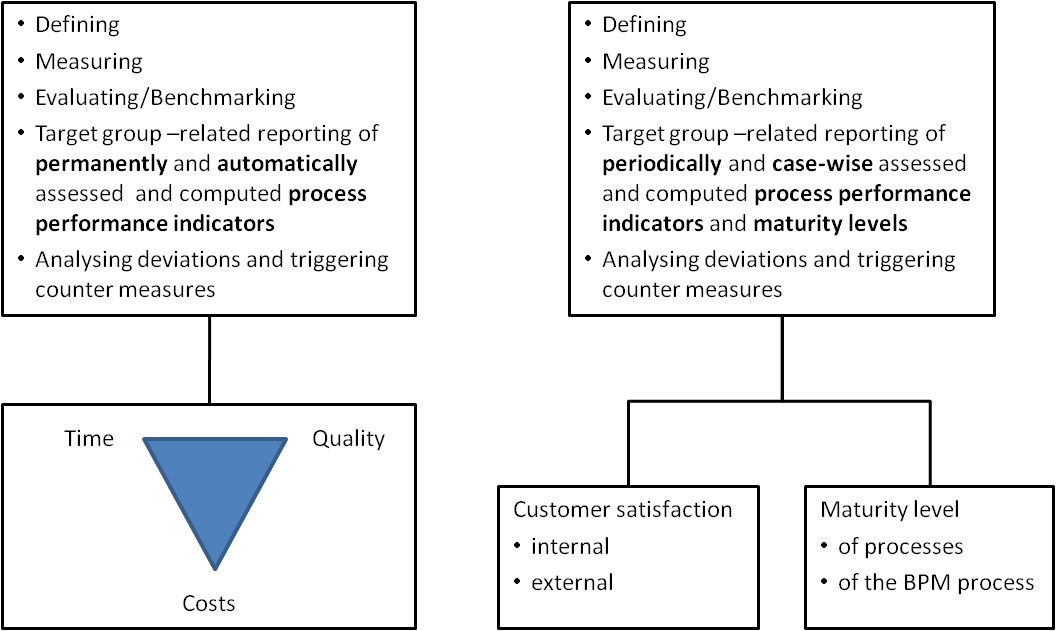
\includegraphics[width=0.6\linewidth] {Figures/Chapter5/ActivityBased/OpProcessCont.jpg}
	\caption[Operational Process Controlling]{Operational Process Controlling}
	\label{fig:OpProcessCont}
\end{figure}

In this section we focus on cost figures. Calculating them is more difficult than assessing those for time and quality. S-BPM allows determining cost figures for processes and process steps as well as for the occupation of cost centers and organizational units with little additional effort though. The reason is that S-BPM specifies subjects as actors in a process, their interaction and their assignment to elements of the organizational structure (organizational units, positions, roles).
\\
The basic methodology to integrate such cost information into process controlling is Activity-Based Costing (ABC).


\subsubsection{Methodology of Activity-Based Costing}
The concept of Activity-Based Costing origins in the work of Miller and Vollmann \cite{article:HiddenFactory} and Cooper and Kaplan \cite{article:MeasureCost} and was established in the German-speaking community by Horvath und Mayer \cite{article:Prozesskosten}.
\\
ABC roots in a simple fact: producing and delivering a product or service involves many activities within cost centers and across boundaries of cost centers or functional areas, all causing costs. Major factors influencing these costs (cost drivers) usually are measures of the activity quantity, e.g. the number of purchasing orders being processed in procurement.
\\
\newline
\textbf{Step 1: Analysing activities}
\\
Starting point for ABC is an analysis of activities performed in the cost centers, using common methods like interviews, questionnaires, self-monitoring, third-party observation, document analysis or multi-moment recording. This analysis is essential for bordering cost center internal process steps and main processes running across cost center boundaries. Self-monitoring and multi-moment recording can bring up time standards for the execution of processes and their steps, but needs high effort. In order to ease the investigation of times, controllers instead often conduct interviews to find out what share of work force capacity the process steps occupy in a cost center.
The analysis results in a transparent, hierarchical process structure showing the assignment of activities to process steps, the assignment of process steps to cost centers and the aggregation of process steps to main processes (cf. figure \ref{fig:ProcessStruct} )

\begin{figure}[htbp]
	\centering
	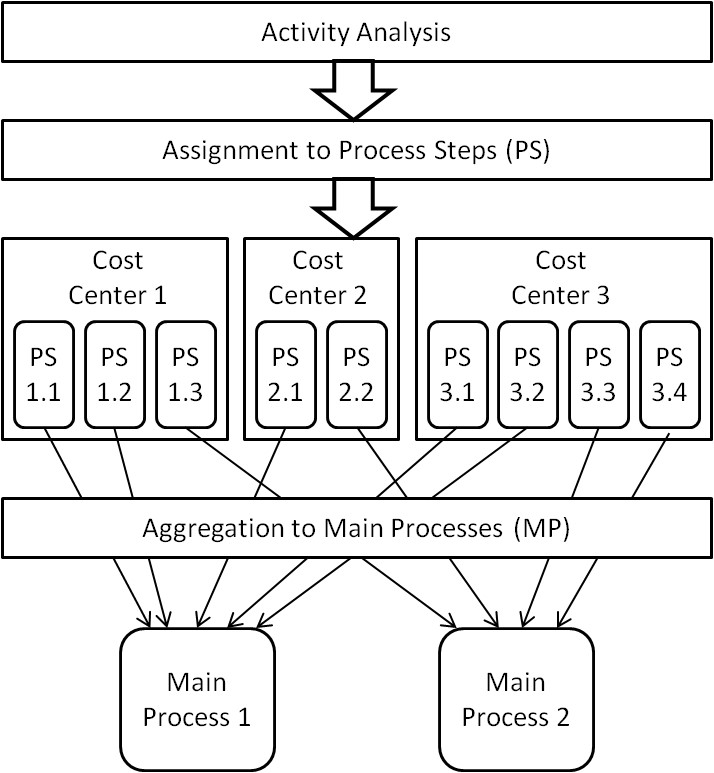
\includegraphics[width=0.6\linewidth] {Figures/Chapter5/ActivityBased/ProcessStruct.jpg}
	\caption[Process Structure]{Process Structure}
	\label{fig:ProcessStruct}
\end{figure}


This first step of Activity-Based Costing can be based on the results of the activity bundles analysis and modeling in S-BPM [6]. ABC-relevant information on subjects, their activities and the business objects being worked on are contained in the S-BPM process model (see section 2.3).
\\
\newline
\textbf{Step 2: Determining cost drivers}
\\
Horvath und Mayer differentiate between activity quantity induced (aqi) and activity quantity neutral (aqi) processes [9]. The latter (e.g. leading a department) cause costs independent from the activity quantity (e.g. the salary of the department leader). In activity quantity induced processes (e.g. purchasing goods) resource consumption and related costs vary with the activity quantity. Hereby process costs incurring depend on the number of cost drivers and there is need to determine measures for those as a second step in ABC. Cost drivers serve as an allocation base for resource utilization and thus also for causing costs.
\\
Cost drivers need to meet some requirements in order to make cost dependence transparent:
\begin{list}{-}{spacing}
	\item Process costs should, at least in the long term, vary with the activity quantity
	\item Cost driver values should be easy to assess and to understand.
	\item Input of resources should be approximately the same for all process instances, otherwise processes and cost drivers need to be further differentiated.
\end{list}

Usually ideas of what the major cost driver is already come up during the activity analysis and the activity quantity can be determined simultaneously then.
\\
\newline
\textbf{Step 3: Determining process costs}
\\
In practice it is often difficult to only assign the major cost driver to the main processes, because a main process can consist of process steps with different cost drivers not being proportionally related.
\\
In a given organizational and cost accounting context resources and costs are planned and actual costs are recorded on cost center level. This means planning and assessing process costs initially is also related to cost centers.
\\
Although theory suggests to plan process costs analytically and by cost type like in direct costing, practitioners prefer more simple concepts. One alternative is to only plan labor costs analytically and to allocate all other cost types proportionally. Another option would be to assign to the analyzed processes the capacities they consume and the related costs. In any case the accountants usually assume the labor cost to be the major cost element. Process costs then can be computed by multiplying a qualified estimate of the number of employees involved in the process by their average wage. If need be activity quantity neutral costs also can be passed on proportionally. In case there are more activity quantity induced costs with a significant extent they need to be considered in addition to labor costs. Even then the described procedure is still easy to handle.
\\
\newline
\textbf{Step 4: Determining process cost rate}
\\
In a last step, for the purpose of job order costing or product calculation, a simple division results in a process cost rate similar to the computation of a machine hour rate.
As shown Activity-Based Costing can be implemented in various ways. The identified problem of different cost drivers that cannot be aggregated can be solved by using time-related allocation bases \cite{article:Rechenzwecke} p. 23.
\\
The concrete process times can be computed if a workflow engine writes time stamps for begin and end events of the process steps. In order to have the engine processing a workflow at runtime, process activities must be assigned to concrete actors. Both kinds of information are needed for establishing ABC as elaborated in section \ref{section:ExampleABC}.


\subsection{BPM as Data Supplier}
Subject-oriented Business Process Management (S-BPM) focuses on the acting elements (actors) and their interactions as they drive a process. Its modeling notation includes all building blocks of a complete sentence in natural language as there are subject, predicate and object. The clear formal semantic of the underlying process algebra makes it possible to automatically generate code and makes subject-oriented process descriptions executable at a finger tip \cite{Flei12}, \cite{article:HMD-S-BPM}.
\\
Major parts of the model are subject interaction diagrams, describing the subjects involved in the process and the messages they exchange, and subject behavior diagrams, specifying subject activities as there are sending and receiving messages and other functions (e.g. manipulating business objects). The ladder means that at a time subjects can either be in a send, receive or functional state.
Transforming the model into a workflow and integrating IT solutions (e.g. ERP functionality) to support particular activities is subject to the embedding of the process into IT. Assigning subjects to elements of the existing organizational structure (organizational units, positions, roles) being responsible for carrying out the activities as defined in the model, is called embedding the process (model) into the organization. Existing directory services based on Lightweight Directory Access Protocol (e.g. Active Directory) can ease the assignment of subjects to roles, groups and people as implemented in Metasonic Suite.
A process engine like Metasonic Flow interprets the model at runtime, instantiates process instances and controls their execution. According to the defined behavior the engine involves users and IT services or applications as subject representatives. It also controls the handling of business objects included the in subject behavior (creation, modification, deletion, exchange through messages). During execution the engine can capture many single pieces of data relevant for process controlling, especially by setting time stamps for state transitions and by counting instances. Examples are

\begin{list}{-}{spacing}
\item begin time and end time of every single instance,
\item begin time and end time of the single steps within an instance or
\item number of instances of a certain process per time unit.
\end{list}
Using such raw data suitable software can compute key figures like
\begin{list}{-}{spacing}
\item waiting time of an instance from the moment it appeared in the in-box of an actor until he or she takes it out for processing (per case, on average) and
\item processing time from taking the instance out of the in-box until putting the result into the out-box (per case, on average).
\end{list}

This means the workflow system generates a valuable data basis for a meaningful Activity-Based Costing. This data needs to be categorized though and the key figures need to be defined precisely and unique in order to derive useful management information (see example in section \ref{section:ExampleABC}).

\subsubsection{Example for Estimating Process Costs in S-BPM} \label{section:ExampleABC}
Effective process controlling, allowing to turn such decisions into the right actions additionally requires information about cost dimensions in processes and cost-related consequences of processes for cost centers. Cost information enables monetary valuation of the enterprise performance as well as identifying weak points in operations and valuating their economic impact.
\\
We exemplify the determination of process costs using an order process. Figure \ref{fig:CalcPro} depicts the behavior diagram for the subject 'purchaser' enriched with some time information. These are times recorded as time stamps for state transitions by the process engine and stored in its event log \cite{article:SubProcessMon}. For clarity reasons in the figure \ref{fig:CalcPro} we only added time stamps for one state and just added the duration for the others.

\begin{figure}[htbp]
	\centering
	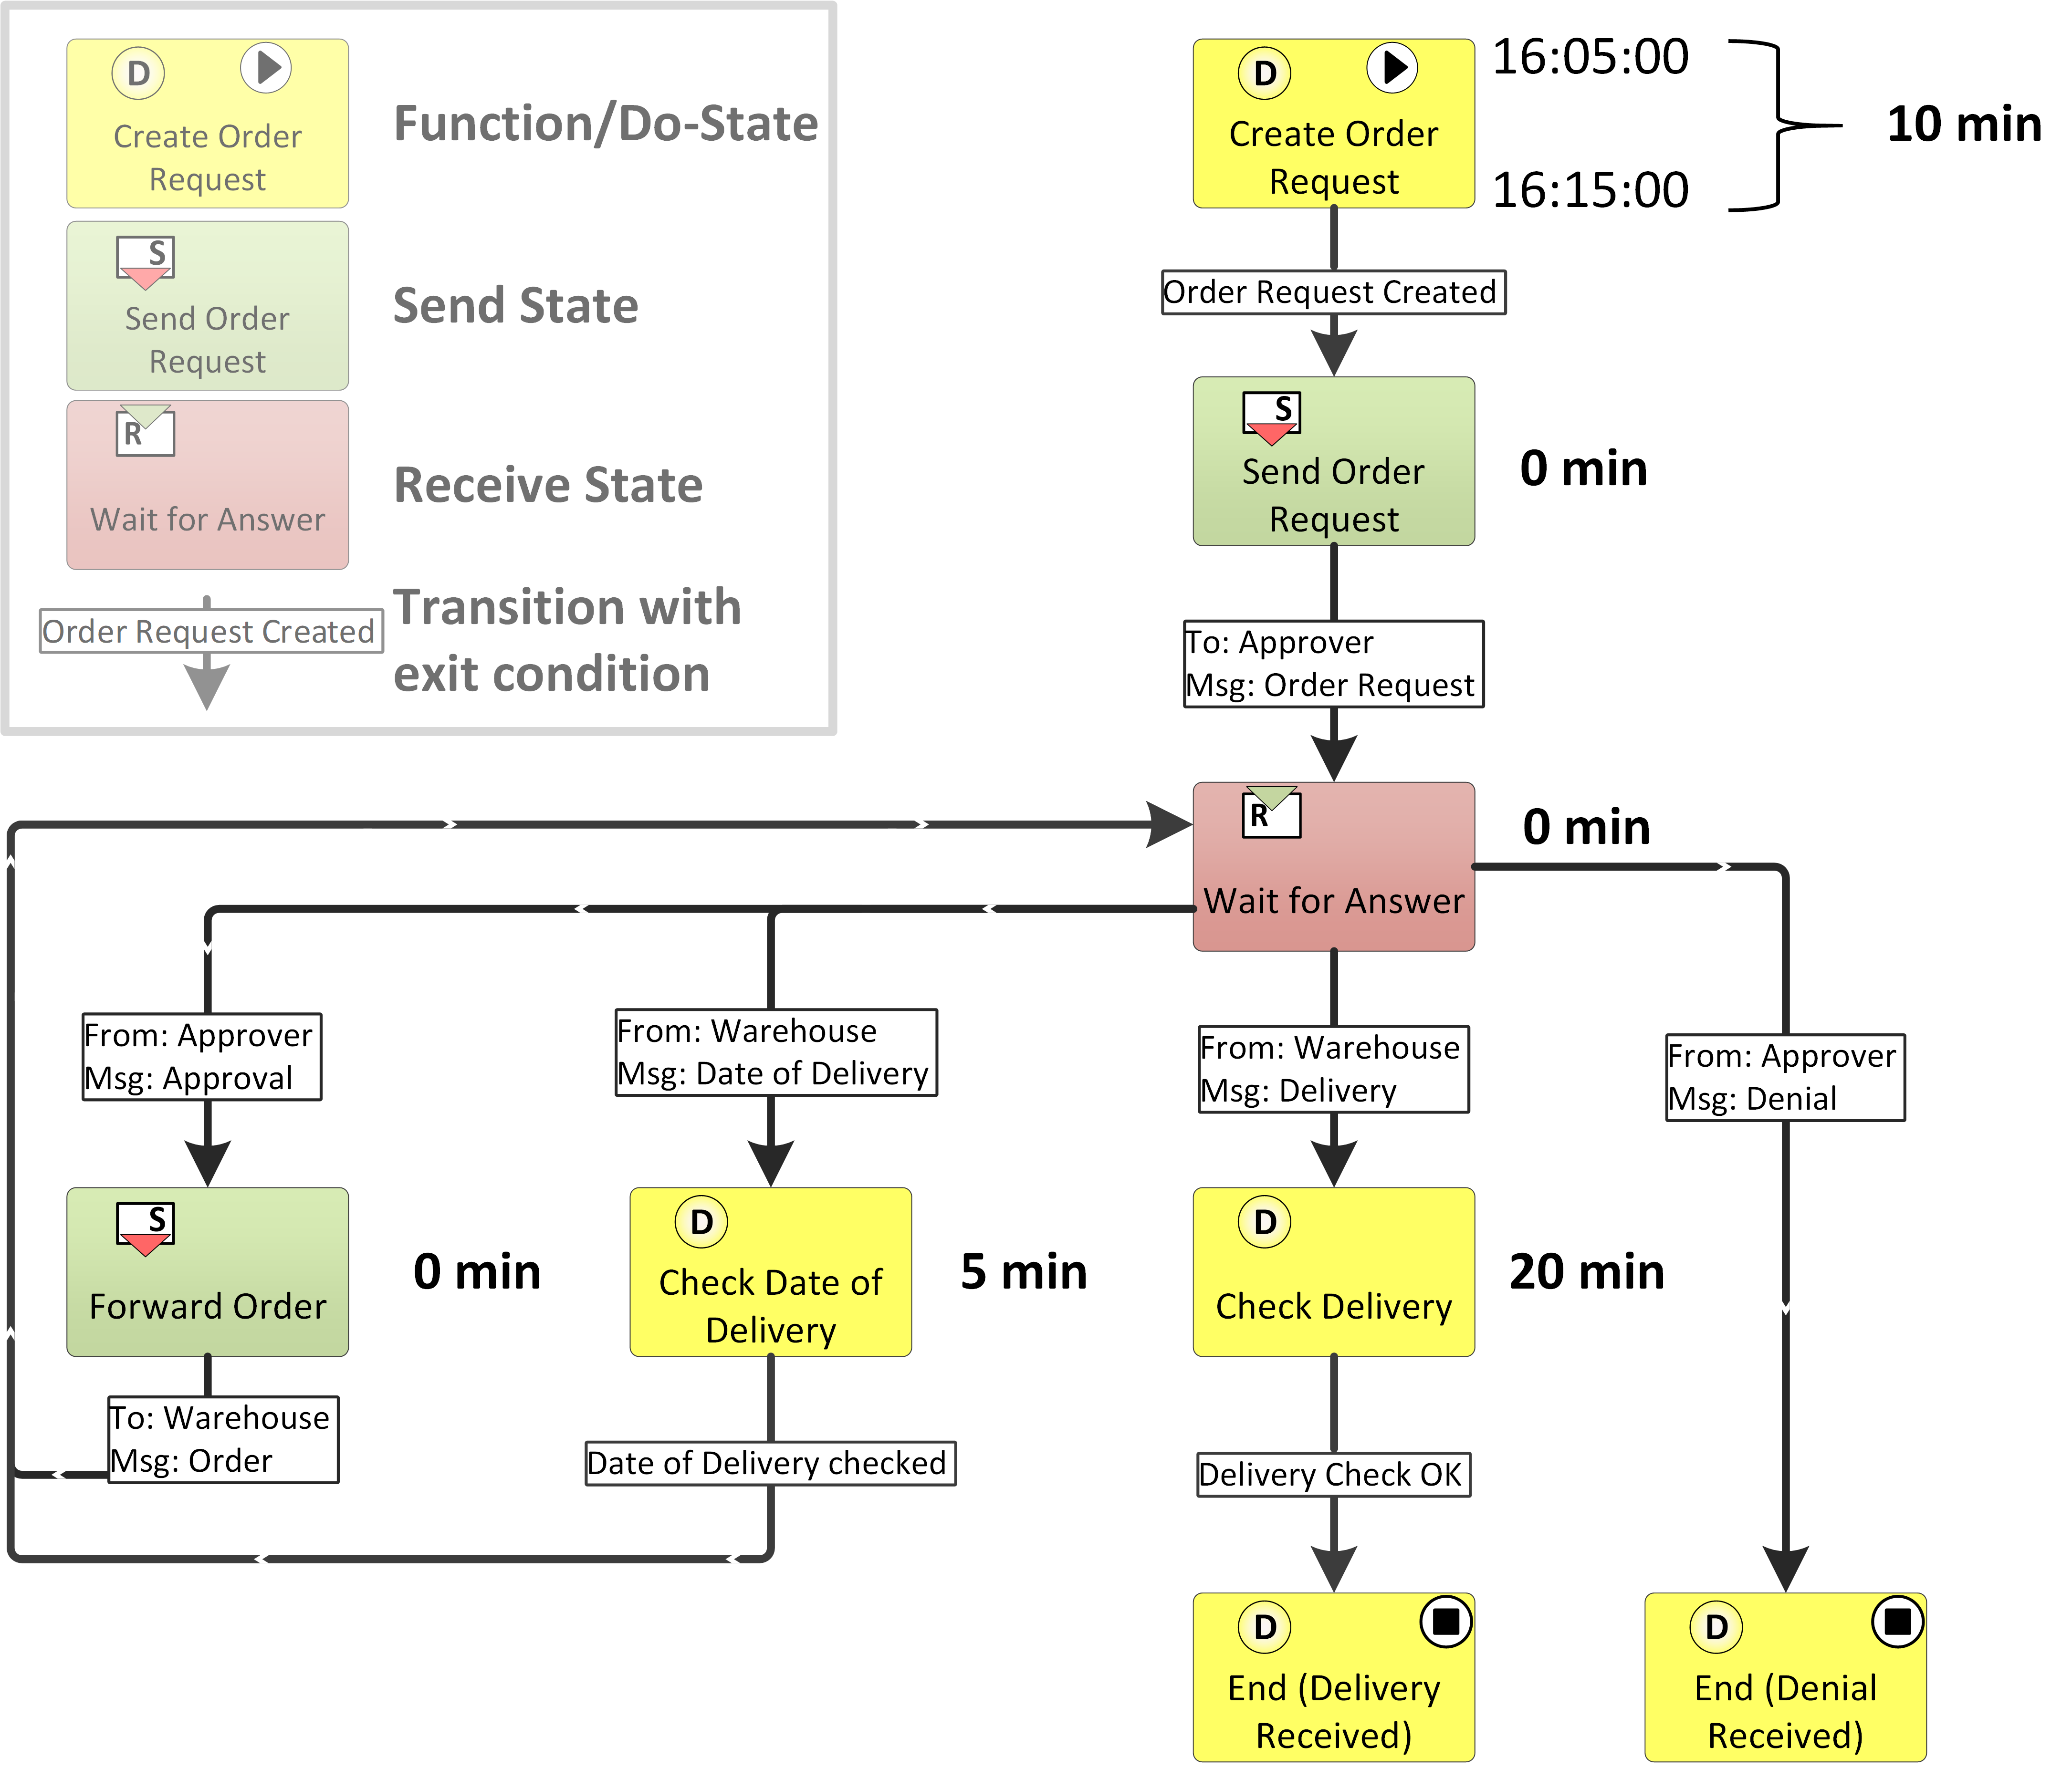
\includegraphics[width=0.6\linewidth] {Figures/Chapter5/ActivityBased/CalcPro_NEW.png}
	\caption[Calculating Processing Time of the Subject 'Purchaser']{Calculating Processing Time of the Subject 'Purchaser'}
	\label{fig:CalcPro}
\end{figure}


In the example the processing time of the subject 'purchaser' in case of the sunshine path (goods are on stock) can be computed by adding up the differences between start and end time of the functional states 'create order request' and 'check delivery'. The sunshine path sequence is as follows: After creating the request the purchaser sends it to the approver and then waits for an answer. If the request is denied the instance ends (right column in figure \ref{fig:CalcPro}). Otherwise the purchaser forwards the request to the warehouse (left column), waits for them to announce the delivery date and checks it (second to left). Finally he waits for the delivery and checks it after reception, before the instance comes to an end (third to left). As a simplification we assume the subject representatives to work permanently when performing functions (being in a functional state). We did not insert times for send and receive states because message exchange is considered to be accomplished electronically with no latency for sending, transmission and receiving. Applying this procedure to all subjects could lead to the result in table \ref{tab:procTime}.

\begin{table}[htbp]
	\centering
\begin{tabular}{|p{5.0 cm } |c|}
\hline
	\textbf{Subject} & Processing Time \\
	\hline
	\hline
	Purchaser & 35 min\\
	\hline
	Approver & 10 min \\
	\hline
	Warehouse & 30 min \\
	\hline
	Invoice Verification & 5 min \\
	\hline
	Accounting/book keeping & 5 min \\
	\hline
	Total & 85 min \\
	\hline
\end{tabular}
\caption{Processing times}
\label{tab:procTime}
\end{table}

For estimating the costs of the process we need an hourly or minute-related rate of wage for the people being assigned to the subjects. It is also possible to provide those values aggregated on group or role level. In Figure 5 we visualized how the subjects in our example are mapped to persons, while table \ref{tab:HourlyWages} gives an overview of the rates for the employees involved as subject representatives.

\begin{figure}[htbp]
	\centering
	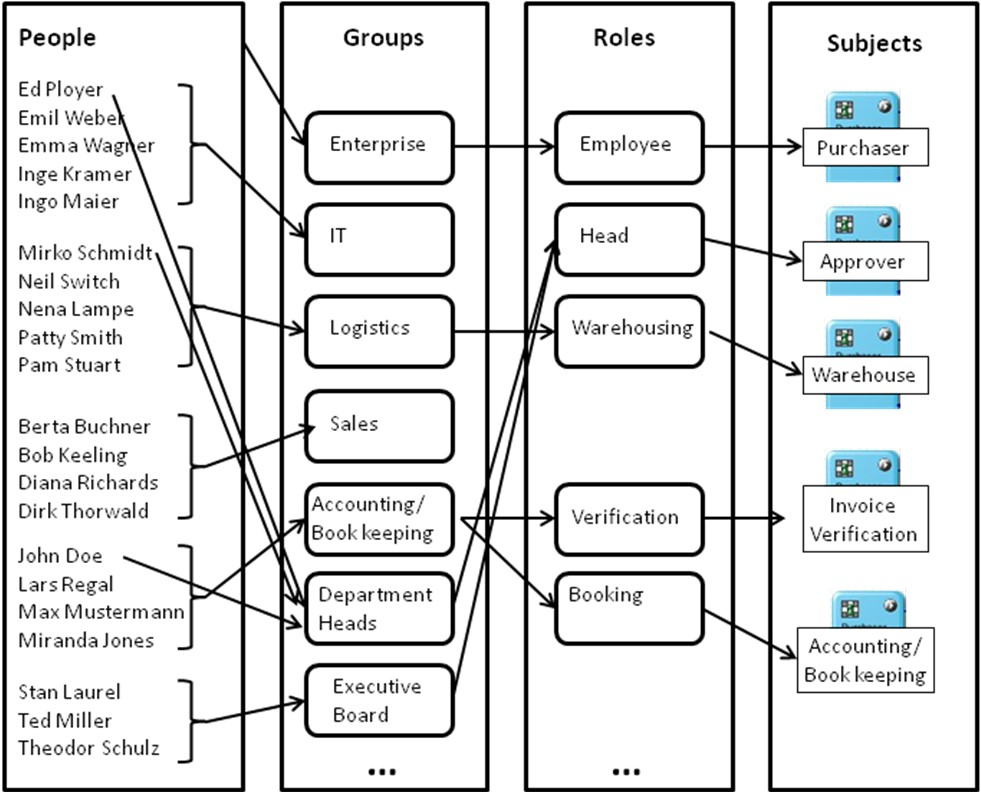
\includegraphics[width=0.6\linewidth] {Figures/Chapter5/ActivityBased/embedding.jpg}
	\caption[Embedding the Subjects into the Organization]{Embedding the Subjects into the Organization}
	\label{fig:Embedding}
\end{figure}

\begin{table}[htbp]
	\centering
	\begin{tabular}{|p{10.0 cm } |c|}
		\hline
		\textbf{Employee} & \textbf{Wage rate} \\
		\hline
		\hline
		Miller, Laurel, Schulz & 200 Euro/hour\\
		\hline
		Ployer, Schmidt, Doe, Keweling & 100 Euro/hour\\
		\hline
		Weber, Wagner, Kramer, Meier, Switch, Lampe, Smith, Stuart, Buchner, Richards, Thorwald, Regal, Mustermann, Jones & 50 Euro/hour\\
		\hline
	\end{tabular}
\caption{Hourly wages rate}
\label{tab:HourlyWages}
\end{table}



Having these time and wage values available it is a simple multiplication to determine the personnel-related process costs for every single instance (cf. table \ref{tab:ProcessCosts}). Considering a sufficient number of instances over a representative period of time allows computing a valid average cost value.

\begin{table}[htbp]
	\centering
	\begin{tabular}{|p{5.0 cm } |c|r|}
		\hline
		\textbf{Subject} & \textbf{Employee} & \textbf{Costs}\\
		\hline
		\hline
		Purchaser & Kramer & 35 Min. x 50 Euro/60 min.  =  29,17 Euro\\
		\hline
		Approver & Ployer & 10 Min. x 100 €/60 min. =  16,67 Euro\\
		\hline
		Warehouse & Lampe & 30 Min. x 50 €/60 min.  =  25,00 Euro\\
		\hline
		Invoice verification & Regal & 5 Min. x 50 €/60 min.    =    4,17 Euro\\
		\hline
		Accounting/Book keeping & Regal & 5 Min. x 50 €/60 min.    =    4,17 Euro\\
		\hline
		Total & & 79,18 Euro\\
		\hline
	\end{tabular}
\caption{Personal Related Process Costs}
\label{tab:ProcessCosts}
\end{table}

Assigning employees as subject representatives embeds the subjects into the organizational structure, because people belong to organizational units. As cost centers usually also are assigned to organizational units it is now possible to determine the costs of a process incurring in a certain cost center. From the cost center perspective it is also possible to see how its total costs are distributed over the processes and process steps it is involved in. Table \ref{tab:CostFig} shows examples for cost figures which can be computed.

\begin{table}[htbp]
	\centering
	\begin{tabular}{|p{3.0 cm } |p{10.0 cm }|}
		\hline
		\textbf{Key figure (Euro)} & \textbf{Computation (e.g. for 10 work days)}\\
		\hline
		\hline
		Process costs per process step/process & Multiply all processing times by the appropriate wage rate and aggregate the products over all instances occurring during the observation period\\
		\hline
		Process costs per cost center & Multiply all processing times incurring in the cost center by the appropriate wage rate and aggregate the products over all instances occurring during the observation period\\
		\hline
	\end{tabular}
\caption{Cost Figures}
\label{tab:CostFig}
\end{table}

As mentioned before key figures need to be defined carefully and precisely. A useful instrument helping to assure this are structured fact sheets being filled in with all necessary information \cite{book:KennzahlenIT}. Table \ref{tab:FactSgeet} depicts such a fact sheet created for our purposes \cite{book:MonitoringSubjekt}. A more formal structure can be found in \cite{article:ProcessPerfInd}.



\begin{table}[htbp]
	\centering
	\begin{tabular}{|p{3.0 cm } |p{10.0 cm }|}
		\hline
		\textbf{Attribute} & \textbf{Content}\\
		\hline
		\hline
		& \textbf{Characteristics}\\
		\hline
		Description & Average costs of a process activity for a certain period\\
		\hline
		To-be value/unit & tbd specifically (Euro)\\
		\hline
		Tolerance range/unit & tbd specifically (\%)\\
		\hline
		Escalation rule & In case of violation alert the process owner and start escalation process (tbd specifically)\\
		\hline
		Responsibility & Process Owner (tbd specifically)\\
		\hline
		\hline
		& \textbf{Measuring and Computing}\\
		\hline
		Measurement & Read time stamps written by Metasonic Flow, compute processing time as difference between time stamps for beginning and end, multiply processing time by hourly wage rate, divide product by number of completed instance\\
		\hline
		Algorithms & Sum up Processing time * hourly wage rate \newline
					Sum up completed instances\\
		\hline
		Data sources(general) & Tables in the database of Metasonic Suite:\newline
		RT\_PROCDESC, RT\_PROCINST, REC\_PARADESC, REC\_RECTRANS, UM\_USER\\
		\hline
		Data sources(specific) & Processing time:\newline
		\hspace*{4mm} \textbf{SELECT} TIMESTAMP1 \newline
		\hspace*{10mm} (\textbf{SELECT} STARTTIME \newline
		\hspace*{10mm} \textbf{FROM} RT\_PROCINST \newline
		\hspace*{10mm} \textbf{WHERE} RT\_PROCDESC = \textit{process} \newline
		\hspace*{10mm} \textbf{AND} ID = \textit{instance} \newline
		\hspace*{4mm}\textbf{FROM} REC\_RECTRANS \newline
		\hspace*{4mm}\textbf{WHERE} RT\_STDESC = \textit{state} \newline
		\hspace*{4mm}\textbf{AND} RT\_PROCINST = \textit{instance} \newline
		Hourly wage rate: UM\_USER (manually enriched by hourly wage rates) \newline
		Completed instances: see separate fact sheet\\
		\hline
		Frequency & weekly\\
		\hline
		\hline
		& \textbf{Presentation} \\
		\hline
		Addressees & Process Owner, Middle Management, Accountants (tbd specifically)\\
		\hline
		Presentation & As-is value and to-be value in combination with a sparkline showing the historical development, deviation from to-be value in \%\\
		\hline
		Archiving & Stored in additional database table, linked with RT\_PROCDESC\\
		\hline
	\end{tabular}
\caption{Fact Sheet for the Key Figure 'Average costs of a process activity'}
\label{tab:FactSgeet}
\end{table}

\subsection{Conclusion}
With the example in chapter 3 we could show that it is relatively easy to integrate cost information into S-BPM. Focusing on personnel costs as suggested avoids the problematic proportioning of costs and therefore is particularly suited for people-intensive areas with a high degree of indirect costs as it is characteristic for services.


\subsection{ Future Work}
A more detailed investigation of how the implementation of Activity-Based Costing can benefit from a preceding S-BPM implementation seems to be promising. Exploiting the conceptual particularities coming with and the data collected by S-BPM seems to bear considerable potential of savings when introducing ABC. Processes are defined and modeled and as-is process quantities per period are available as well as the distribution of the overall capacity of the cost centers over the process steps. These parameters allow determining a standard time for processes which lays the ground for planning process costs.
Next steps could be to extend the example by determining and specifying more key figures and testing them with representative numbers of instances of different processes. Learning from this could help to further elaborate the ABC concept for S-BPM.\\
The OWL specification has to be extended with features which support Activity based costing. This includes the data which should be collected and the structure in which these data are stored.
